\documentclass[12pt]{article}


\usepackage{amssymb}
\usepackage{amsmath}
\usepackage{fullpage}
\usepackage{epsfig}
\usepackage{epstopdf}
\everymath{\displaystyle}
\usepackage{enumerate}



\begin{document}

\begin{center}
\underline{\LARGE{Polar Coordinates: Tangent Lines, Arc Length, \& Area}}
\end{center}

\noindent SUGGESTED REFERENCE MATERIAL:

\bigskip

\noindent As you work through the problems listed below, you should reference Chapter 10.3 of the recommended textbook (or the equivalent chapter in your alternative textbook/online resource) and your lecture notes.

\bigskip

\noindent EXPECTED SKILLS:

\begin{itemize}

\item Know how to compute the slope of the tangent line to a polar curve at a given point. 

\item Be able to find the arc length of a polar curve.

\item Be able to Calculate the area enclosed by a polar curve or curves.

\end{itemize}

\noindent PRACTICE PROBLEMS:

\medskip

\noindent {\bf For problems 1-3, find the slope of the tangent line to the polar curve for the given value of $\theta$.}

\begin{enumerate}

\item $r=\theta$; $\theta=\frac{\pi}{6}$ 

\includegraphics[scale=0.5]{start.pdf}
{{$\frac{\sqrt{3}\pi+6}{6\sqrt{3}-\pi}$}}
\includegraphics[scale=0.5]{end.pdf}


\item $r=3+2\sin{\theta}$; $\theta=\frac{\pi}{6}$ 

\includegraphics[scale=0.5]{start.pdf}
{{$-5\sqrt{3}$}}
\includegraphics[scale=0.5]{end.pdf}


\item $r=1-\sin{2\theta}$; $\theta = \pi$ 

\includegraphics[scale=0.5]{start.pdf}
{{$\frac{1}{2}$}}
\includegraphics[scale=0.5]{end.pdf}


\item Consider the circle $r=3\cos{\theta}$.  Find all values of $\theta$ in $0 \leq \theta < \pi$ for which the curve has either a horizontal or vertical tangent line.

\includegraphics[scale=0.5]{start.pdf}
{{{1\linewidth}{Vertical Tangent Lines when $\theta=0$ and $\theta=\frac{\pi}{2}$;\\ Horizontal Tangent Lines when $\theta=\frac{\pi}{4}$ or $\theta=\frac{3\pi}{4}$.}}}
\includegraphics[scale=0.5]{end.pdf}


\end{enumerate}

\noindent {\bf For problems 5-7, fnd the arc length of the given curves}

\begin{enumerate}
\setcounter{enumi}{4}

\item The entire circle $r=4\sin{\theta}$.

\includegraphics[scale=0.5]{start.pdf}
{{$4\pi$}}
\includegraphics[scale=0.5]{end.pdf}


\item The spiral $r=e^{-\theta}$ for $\theta \geq 0$.

\includegraphics[scale=0.5]{start.pdf}
{{$\sqrt{2}$}}
\includegraphics[scale=0.5]{end.pdf}


\item The entire cardioid $r=1+\cos{\theta}$. (Hint: It may be useful to use symmetry and the identity $\cos^2{\theta}=\frac{1}{2}(1+\cos{(2\theta)}$)

\includegraphics[scale=0.5]{start.pdf}
{{8}}
\includegraphics[scale=0.5]{end.pdf}


\end{enumerate}

\noindent {\bf For problems 8-16, find the area of each of the specified regions.}

\begin{enumerate}
\setcounter{enumi}{7}

\item The region in the 1st quadrant within the circle $r=3\cos{\theta}$ 

\includegraphics[scale=0.5]{start.pdf}
{{$\frac{9\pi}{8}$}}
\includegraphics[scale=0.5]{end.pdf}


\item The region enclosed by the cardioid $r=3+3\sin{\theta}$ 

\includegraphics[scale=0.5]{start.pdf}
{{$\frac{27\pi}{2}$}}
\includegraphics[scale=0.5]{end.pdf}


\item The region inside the circle $r=3$ but outside the cardioid $r=1+\cos{\theta}$ 

\includegraphics[scale=0.5]{start.pdf}
{{$\frac{15\pi}{2}$}}
\includegraphics[scale=0.5]{end.pdf}


\item The region inside the circle $r=3$ but outside the cardioid $r=2+2\cos{\theta}$ 

\includegraphics[scale=0.5]{start.pdf}
{{$\frac{9\sqrt{3}}{2}+2\pi$}}
\includegraphics[scale=0.5]{end.pdf}


\item The region outside the circle $r=3$ but inside the cardioid $r=2+2\cos{\theta}$ 

\includegraphics[scale=0.5]{start.pdf}
{{$\frac{9\sqrt{3}}{2}-\pi$}}
\includegraphics[scale=0.5]{end.pdf}


\item The region in common between the two circles $r=3\sin{\theta}$ and $r=3\cos{\theta}$ 

\includegraphics[scale=0.5]{start.pdf}
{{$-\frac{9}{4}+\frac{9\pi}{8}$}}
\includegraphics[scale=0.5]{end.pdf}


\item The region inside the circle $r=2$ and to the right of the line $r=\sec{\theta}$ 

\includegraphics[scale=0.5]{start.pdf}
{{$\frac{4\pi}{3}-\sqrt{3}$}}
\includegraphics[scale=0.5]{end.pdf}


\item The region enclosed by the rose $r=3\cos{2\theta}$ 

\includegraphics[scale=0.5]{start.pdf}
{{$\frac{9\pi}{2}$}}
\includegraphics[scale=0.5]{end.pdf}


\item The region enclosed by the rose $r=2\sin{3\theta}$ 

\includegraphics[scale=0.5]{start.pdf}
{{$\pi$}}
\includegraphics[scale=0.5]{end.pdf}


\item Find the area of the shaded region (shown below) which is enclosed between the circle $r=2\cos{\theta}$ and the cardioid $r=2+2\cos{\theta}$.

\begin{center}
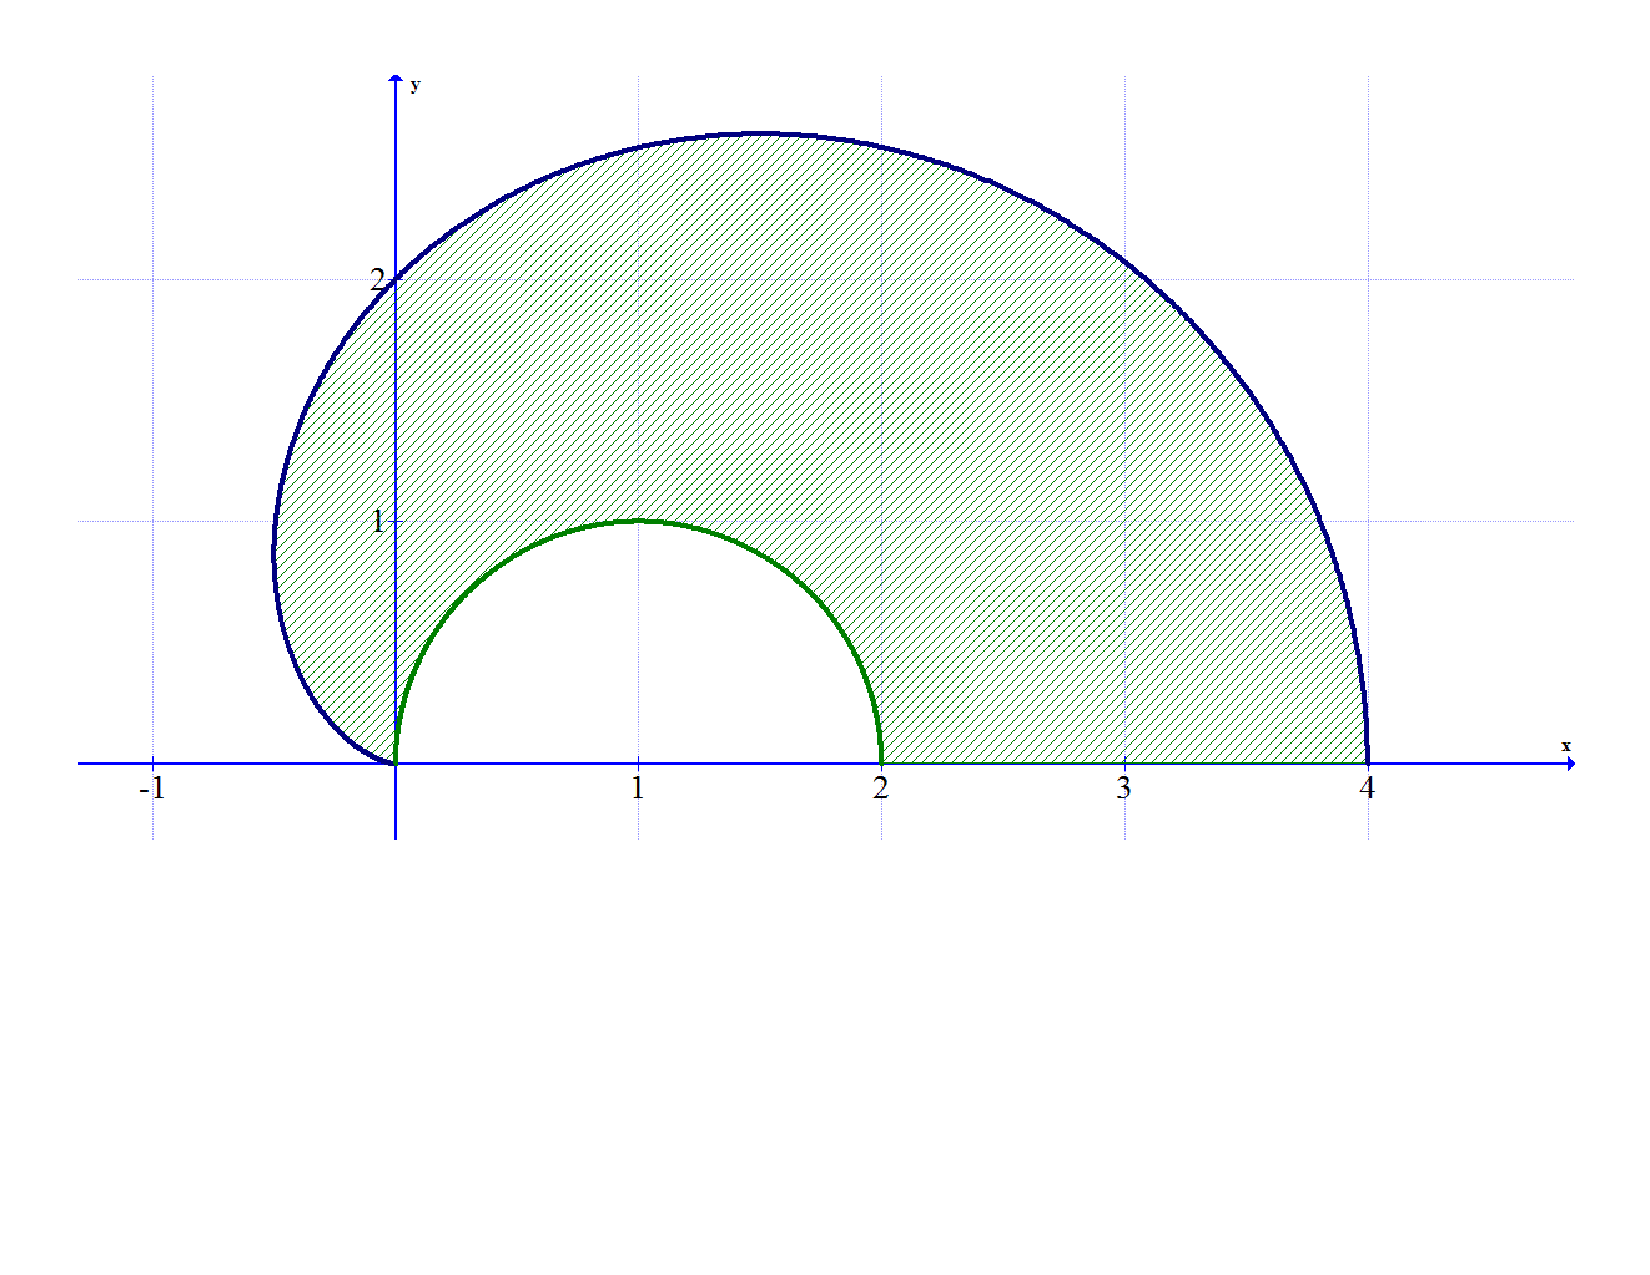
\includegraphics[scale=0.4]{area.pdf}
\end{center}

\includegraphics[scale=0.5]{start.pdf}
{{$\frac{5\pi}{2}$}}
\includegraphics[scale=0.5]{end.pdf}


\item Consider the lima\c{c}on $r=\sqrt{3}+2\sqrt{3}\cos{\theta}$

\begin{center}
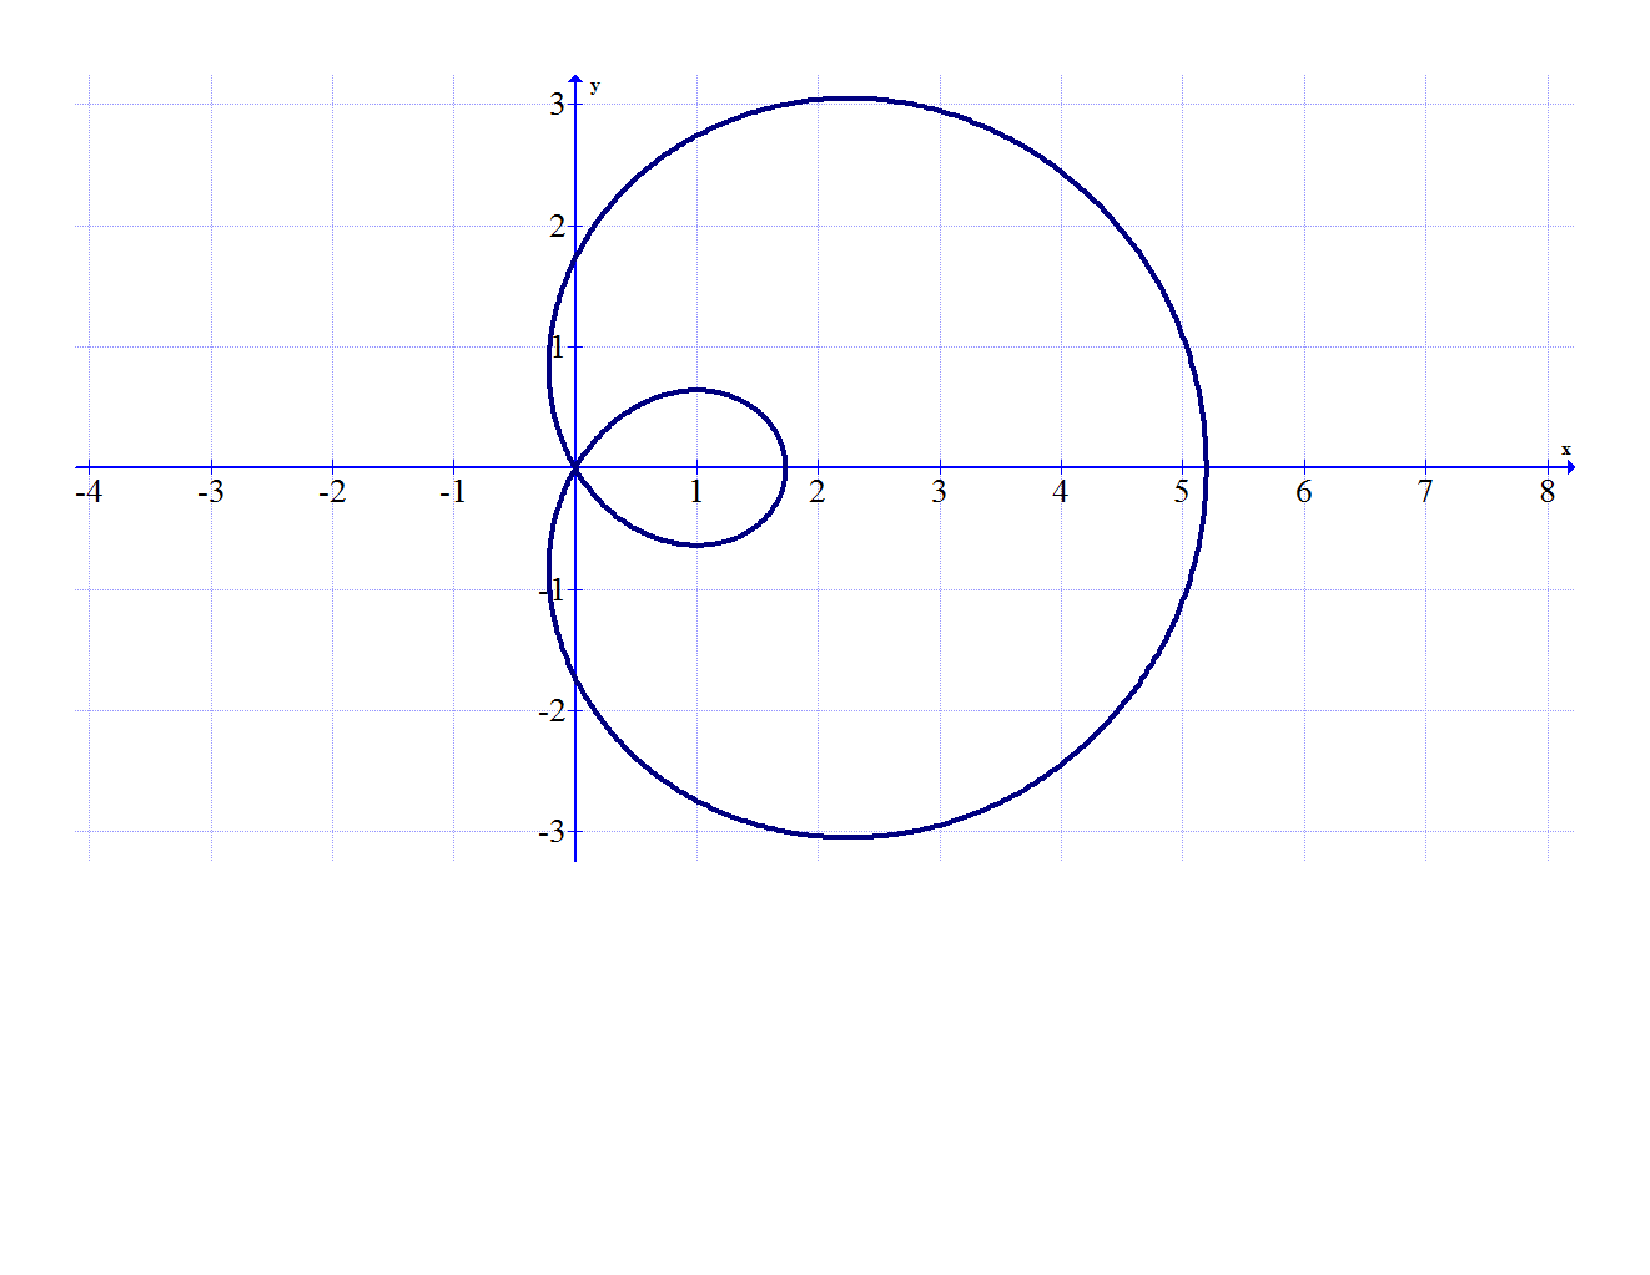
\includegraphics[scale=0.5]{limacon}
\end{center}

\begin{enumerate}

\item Compute the area enclosed by the inner loop of the limacon.

\includegraphics[scale=0.5]{start.pdf}
{{$-\frac{9\sqrt{3}}{2}+3\pi$}}
\includegraphics[scale=0.5]{end.pdf}


\item Compute the area enclosed between the outer and inner loops of the limacon.

\includegraphics[scale=0.5]{start.pdf}
{{$9\sqrt{3}+3\pi$}}
\includegraphics[scale=0.5]{end.pdf}


\end{enumerate}

\end{enumerate}

\end{document}